\documentclass[11pt,a4paper]{article}
\usepackage{../common/polycopie_style}

\begin{document}

\makepolycopieheader{Régression Non Linéaire \& Modélisation Enzymatique}{Cinétiques de Saturation, Algorithmes d'Optimisation \& Modèles Sigmoïdes}{CHAPITRE 4}

\section{Introduction : La Non-Linéarité Fondamentale du Vivant}

En biochimie et physiologie cellulaire, les phénomènes biologiques ne sont presque jamais linéaires :
\begin{itemize}[leftmargin=*, label=\faAngleRight]
  \item \textbf{Saturation des sites catalytiques :} Une enzyme ne peut pas accélérer indéfiniment une réaction ; à haute concentration en substrat, tous les sites actifs sont occupés ($V_{\max}$).
  \item \textbf{Fixation récepteur-ligand :} L'interaction obéit à la loi d'action de masse (équation de Langmuir-Hill).
  \item \textbf{Régulation allostérique :} La transition coopérative entre états relâché (R) et tendu (T) confère aux enzymes clés une réponse sigmoïde ultraréactive.
\end{itemize}

\begin{conceptbox}{Le Principe de la Régression Non Linéaire (NLLS)}
Contrairement à la régression linéaire où les paramètres $a$ et $b$ se calculent directement par des formules algébriques closes, en régression non linéaire, \textbf{il n'existe aucune solution analytique directe}. Les paramètres sont estimés de manière itérative par des algorithmes numériques d'optimisation (Gauss-Newton, Levenberg-Marquardt).
\end{conceptbox}

\section{Le Modèle de Michaelis-Menten}

Pour une réaction enzymatique mono-substrat $E + S \rightleftharpoons ES \rightarrow E + P$, la vitesse initiale $v$ obéit à l'équation hyperbolique :
\begin{equation*}
  v = \frac{V_{\max} \cdot [S]}{K_m + [S]}
\end{equation*}

\begin{biobox}{Signification Biologique des Deux Paramètres}
\begin{itemize}[leftmargin=*, label=\faCheck]
  \item \textbf{Vitesse Maximale ($V_{\max}$) :} Activité catalytique théorique lorsque toutes les molécules d'enzyme sont saturées sous forme de complexe $ES$ ($V_{\max} = k_{\text{cat}} [E]_T$). Elle dépend de la quantité d'enzyme présente.
  \item \textbf{Constante de Michaelis ($K_m$) :} Concentration en substrat pour laquelle $v = \frac{V_{\max}}{2}$. Elle est \textbf{inversement proportionnelle à l'affinité apparente} de l'enzyme :
  \begin{equation*}
    \text{Un } K_m \text{ faible} \iff \text{Forte affinité (l'enzyme est saturée à très faible dose)}
  \end{equation*}
\end{itemize}
\end{biobox}

\section{L'Écueil Historique de la Linéarisation de Lineweaver-Burk}

Avant l'avènement des ordinateurs, les biochimistes inversaient mathématiquement l'équation de Michaelis-Menten :
\begin{equation*}
  \frac{1}{v} = \frac{K_m}{V_{\max}} \cdot \frac{1}{[S]} + \frac{1}{V_{\max}}
\end{equation*}

\begin{warnbox}{Pourquoi Lineweaver-Burk est Désormais Interdit dans les Publications}
La transformation en double réciproque induit une \textbf{distorsion dramatique de l'erreur expérimentale} :
\begin{itemize}[leftmargin=*, label=\faTimesCircle]
  \item Les points à faibles concentrations ($[S]$ petit $\implies 1/[S]$ grand), qui sont techniquement les plus imprécis, se retrouvent rejetés à l'extrême droite du graphique et dominent artificiellement le calcul de la pente !
  \item L'erreur résiduelle n'est plus du tout constante (violation totale de l'homoscédasticité).
\end{itemize}
$\implies$ Les revues scientifiques internationales exigent aujourd'hui l'ajustement direct non linéaire par Moindres Carrés Ordinaires (NLLS).
\end{warnbox}

\begin{figurebox}{Comparaison Visuelle : Ajustement Direct NLLS vs Linéarisation Lineweaver-Burk}
\begin{center}
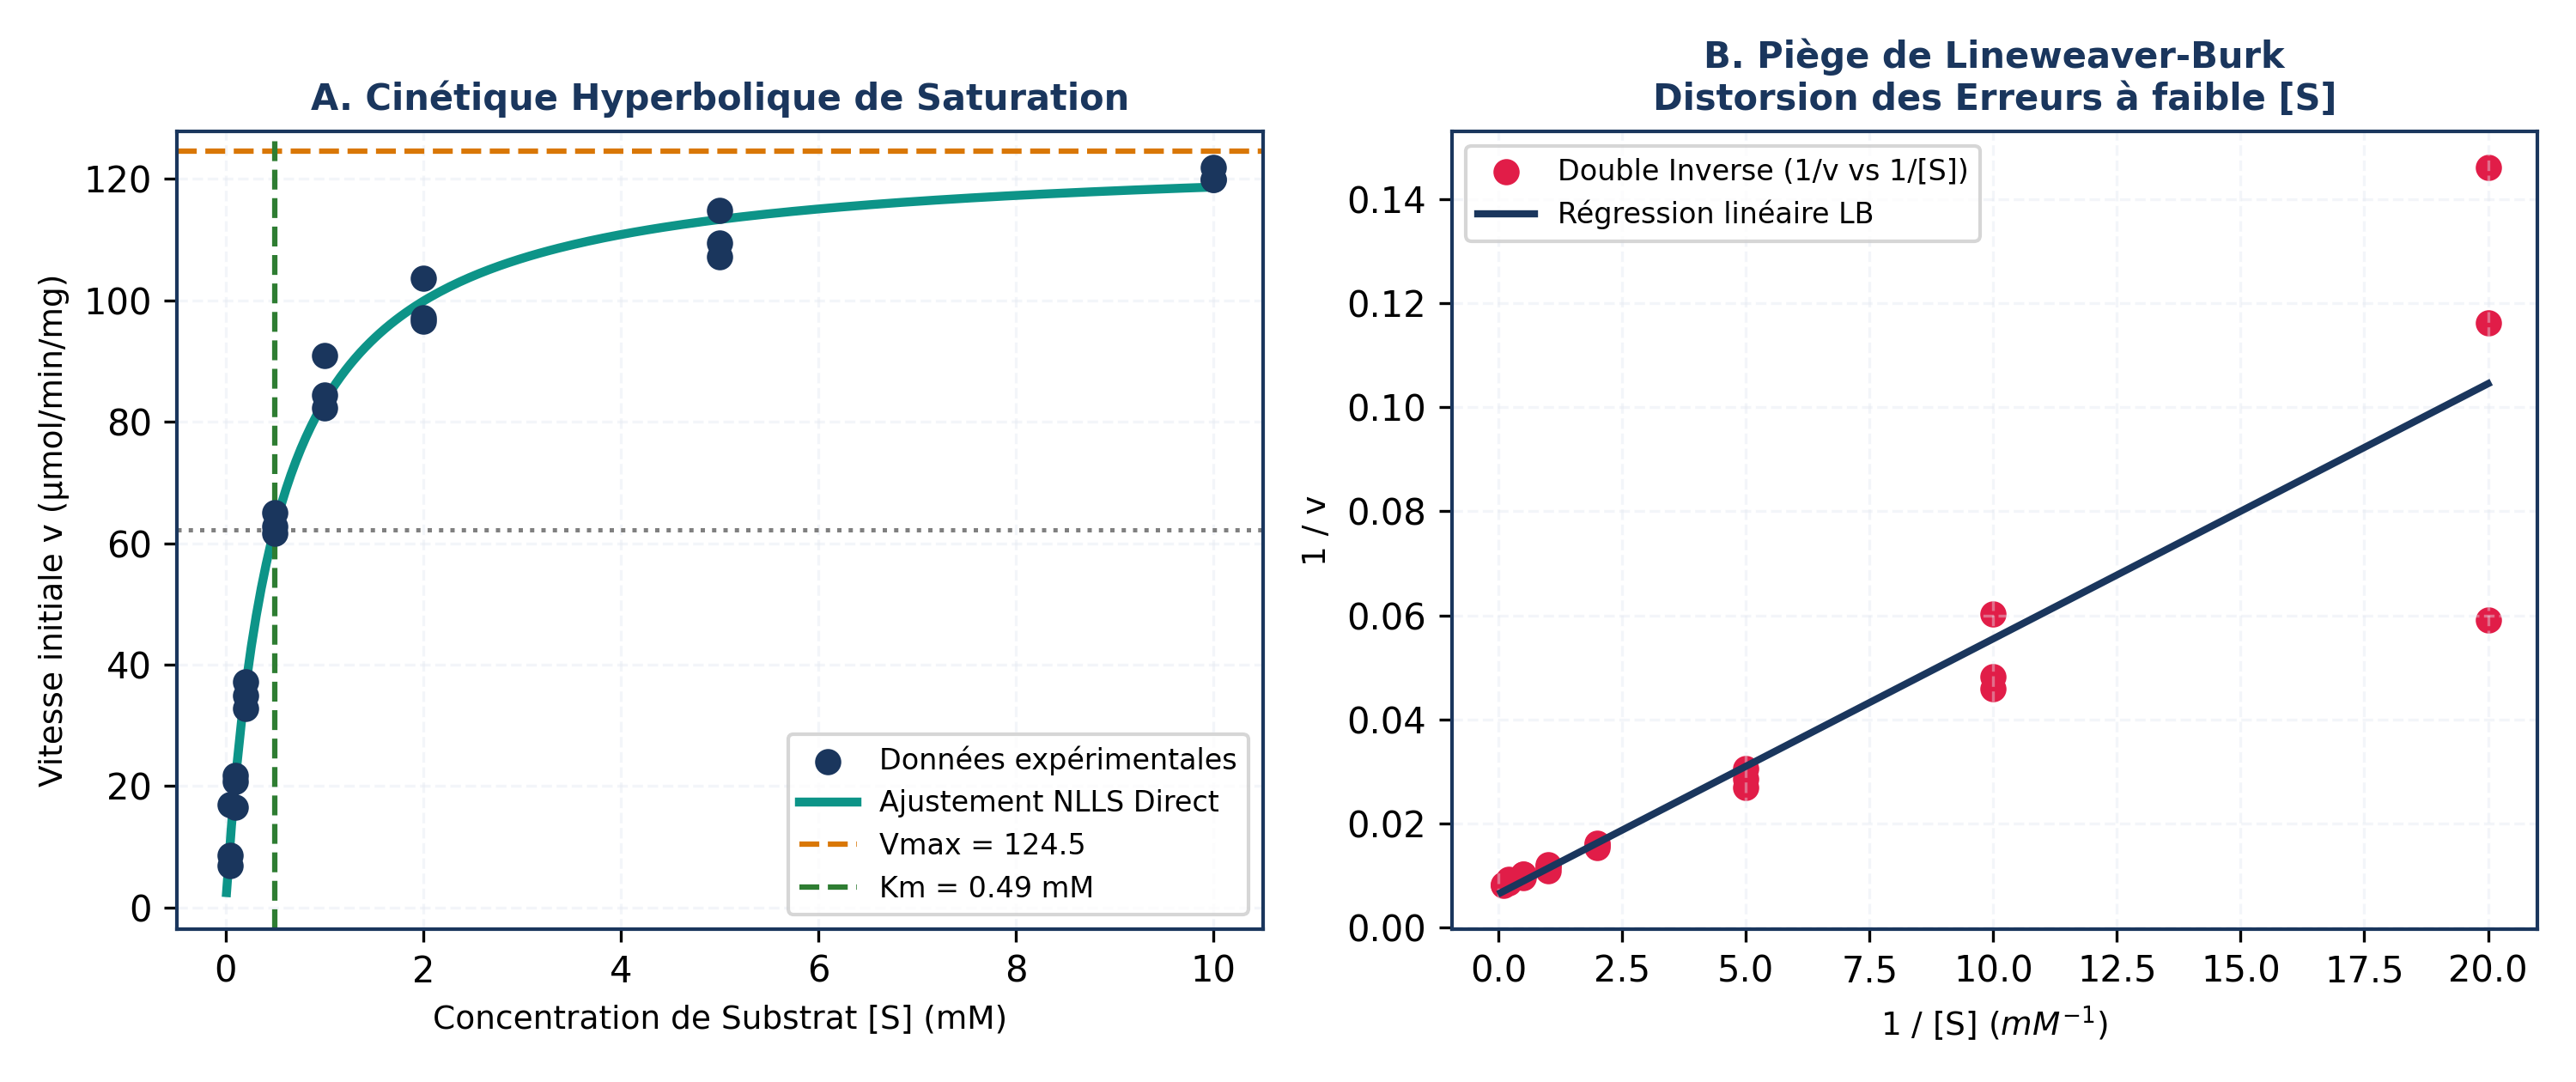
\includegraphics[width=0.86\linewidth]{../../sources/figures/fig04_nlls_vs_lineweaver_burk.png}
\end{center}
\textbf{Analyse comparative des deux approches :}
\begin{itemize}[leftmargin=*, label=\faAngleRight]
  \item \textbf{Graphique de Gauche (Ajustement Direct NLLS) :} L'hyperbole de Michaelis-Menten est ajustée directement sur les données réelles $[S]$ vs $v$. Les barres d'erreur restent uniformes et les bandes de confiance à 95\% reflètent la véritable précision expérimentale sans altération.
  \item \textbf{Graphique de Droite (Double Réciproque de Lineweaver-Burk) :} En inversant $1/[S]$ et $1/v$, les barres d'erreur minuscules à forte concentration sont comprimées près de l'origine, tandis que les barres d'erreur à faible concentration sont disproportionnellement étirées. Une infime imprécision sur le premier point fait basculer toute la droite, faussant lourdement $V_{\max}$ et $K_m$.
\end{itemize}
\end{figurebox}

\section{Algorithme de Levenberg-Marquardt \& Inférence NLLS}

L'algorithme NLLS cherche le vecteur de paramètres $\hat{\theta} = (\hat{V}_{\max}, \hat{K}_m)^T$ qui minimise la somme des carrés des résidus :
\begin{equation*}
  SS_{\text{res}}(\theta) = \sum_{i=1}^n \left( v_i - f([S]_i; \theta) \right)^2
\end{equation*}

L'algorithme de \textbf{Levenberg-Marquardt (LM)} est un standard d'ingénierie qui résout le système itératif :
\begin{equation*}
  \left( J^T J + \lambda \, \text{diag}(J^T J) \right) \Delta \theta = J^T (y - \hat{y})
\end{equation*}
où $J$ est la matrice Jacobienne des dérivées partielles ($\partial f / \partial \theta_j$) et $\lambda$ le paramètre d'amortissement :
\begin{enumerate}[leftmargin=*, label=\faCheck\ \textbf{\arabic*.}]
  \item \textbf{Si $\lambda$ est grand :} L'algorithme se comporte comme une \textbf{descente de gradient} pure, idéale pour s'approcher du minimum global même avec des estimations initiales grossières.
  \item \textbf{Si $\lambda \rightarrow 0$ :} L'algorithme bascule vers la méthode de \textbf{Gauss-Newton}, assurant une convergence quadratique ultra-rapide au voisinage immédiat de la solution optimale.
\end{enumerate}

La matrice de covariance asymptotique des paramètres s'obtient par l'inverse de la matrice d'information de Fisher :
\begin{equation*}
  \widehat{\text{Cov}}(\hat{\theta}) = s^2 \cdot (J^T J)^{-1} \quad \text{avec} \quad s^2 = \frac{SS_{\text{res}}}{n - p}
\end{equation*}
Les racines carrées des éléments diagonaux fournissent les erreurs-types asymptotiques $SE(V_{\max})$ et $SE(K_m)$, permettant de dresser les intervalles de confiance à 95\% :
\begin{equation*}
  IC_{95\%}(K_m) = \left[ \hat{K}_m \pm t_{0.05}(n - 2) \cdot SE(K_m) \right]
\end{equation*}

\section{Coopérativité Allostérique \& Modèle de Hill}

Pour les enzymes oligomériques à sous-unités multiples (ex : Phosphofructokinase, Hémoglobine), la cinétique devient sigmoïde et obéit au modèle de Hill :
\begin{equation*}
  v = \frac{V_{\max} \cdot [S]^{n_H}}{K_{0.5}^{n_H} + [S]^{n_H}}
\end{equation*}
\begin{itemize}[leftmargin=*, label=\faAngleRight]
  \item \textbf{$n_H > 1$ (Coopérativité positive) :} La fixation d'un premier substrat facilite la fixation des suivants. La réponse passe rapidement de 0 à $V_{\max}$ (effet d'interrupteur biochimique).
  \item \textbf{$n_H = 1$ :} Cas limite michaelien (absence d'allostérie).
  \item \textbf{$n_H < 1$ (Coopérativité négative) :} La fixation du premier ligand défavorise les sites voisins.
\end{itemize}

\section{Modèle Logistique à 4 Paramètres (4PL) en Immuno-Analyse (ELISA)}

Dans les dosages immunologiques de type ELISA, ECLIA ou Luminex, la liaison anticorps-antigène suit une réponse sigmoïde en échelle logarithmique de concentration, modélisée par l'équation \textbf{4PL (Four-Parameter Logistic)} :
\begin{equation*}
  Y = D + \frac{A - D}{1 + \left( \frac{X}{C} \right)^B}
\end{equation*}
\begin{itemize}[leftmargin=*, label=\faCheck]
  \item \textbf{$A$ (Asymptote inférieure / Bruit de fond) :} Signal optique théorique en l'absence totale d'analyte ($X = 0$).
  \item \textbf{$D$ (Asymptote supérieure / Saturation) :} Signal optique maximal à saturation complète des puits par l'anticorps.
  \item \textbf{$C$ (Point d'inflexion / $EC_{50}$) :} Concentration d'analyte produisant $50\%$ du signal spécifique utile ($Y = \frac{A+D}{2}$).
  \item \textbf{$B$ (Pente de Hill / Facteur de forme) :} Pente relative au point d'inflexion ; détermine la dynamique de la plage utile de mesure.
\end{itemize}

\begin{figurebox}{Courbes Sigmoïdes : Modèle 4PL (ELISA) \& Allostérie de Hill}
\begin{center}
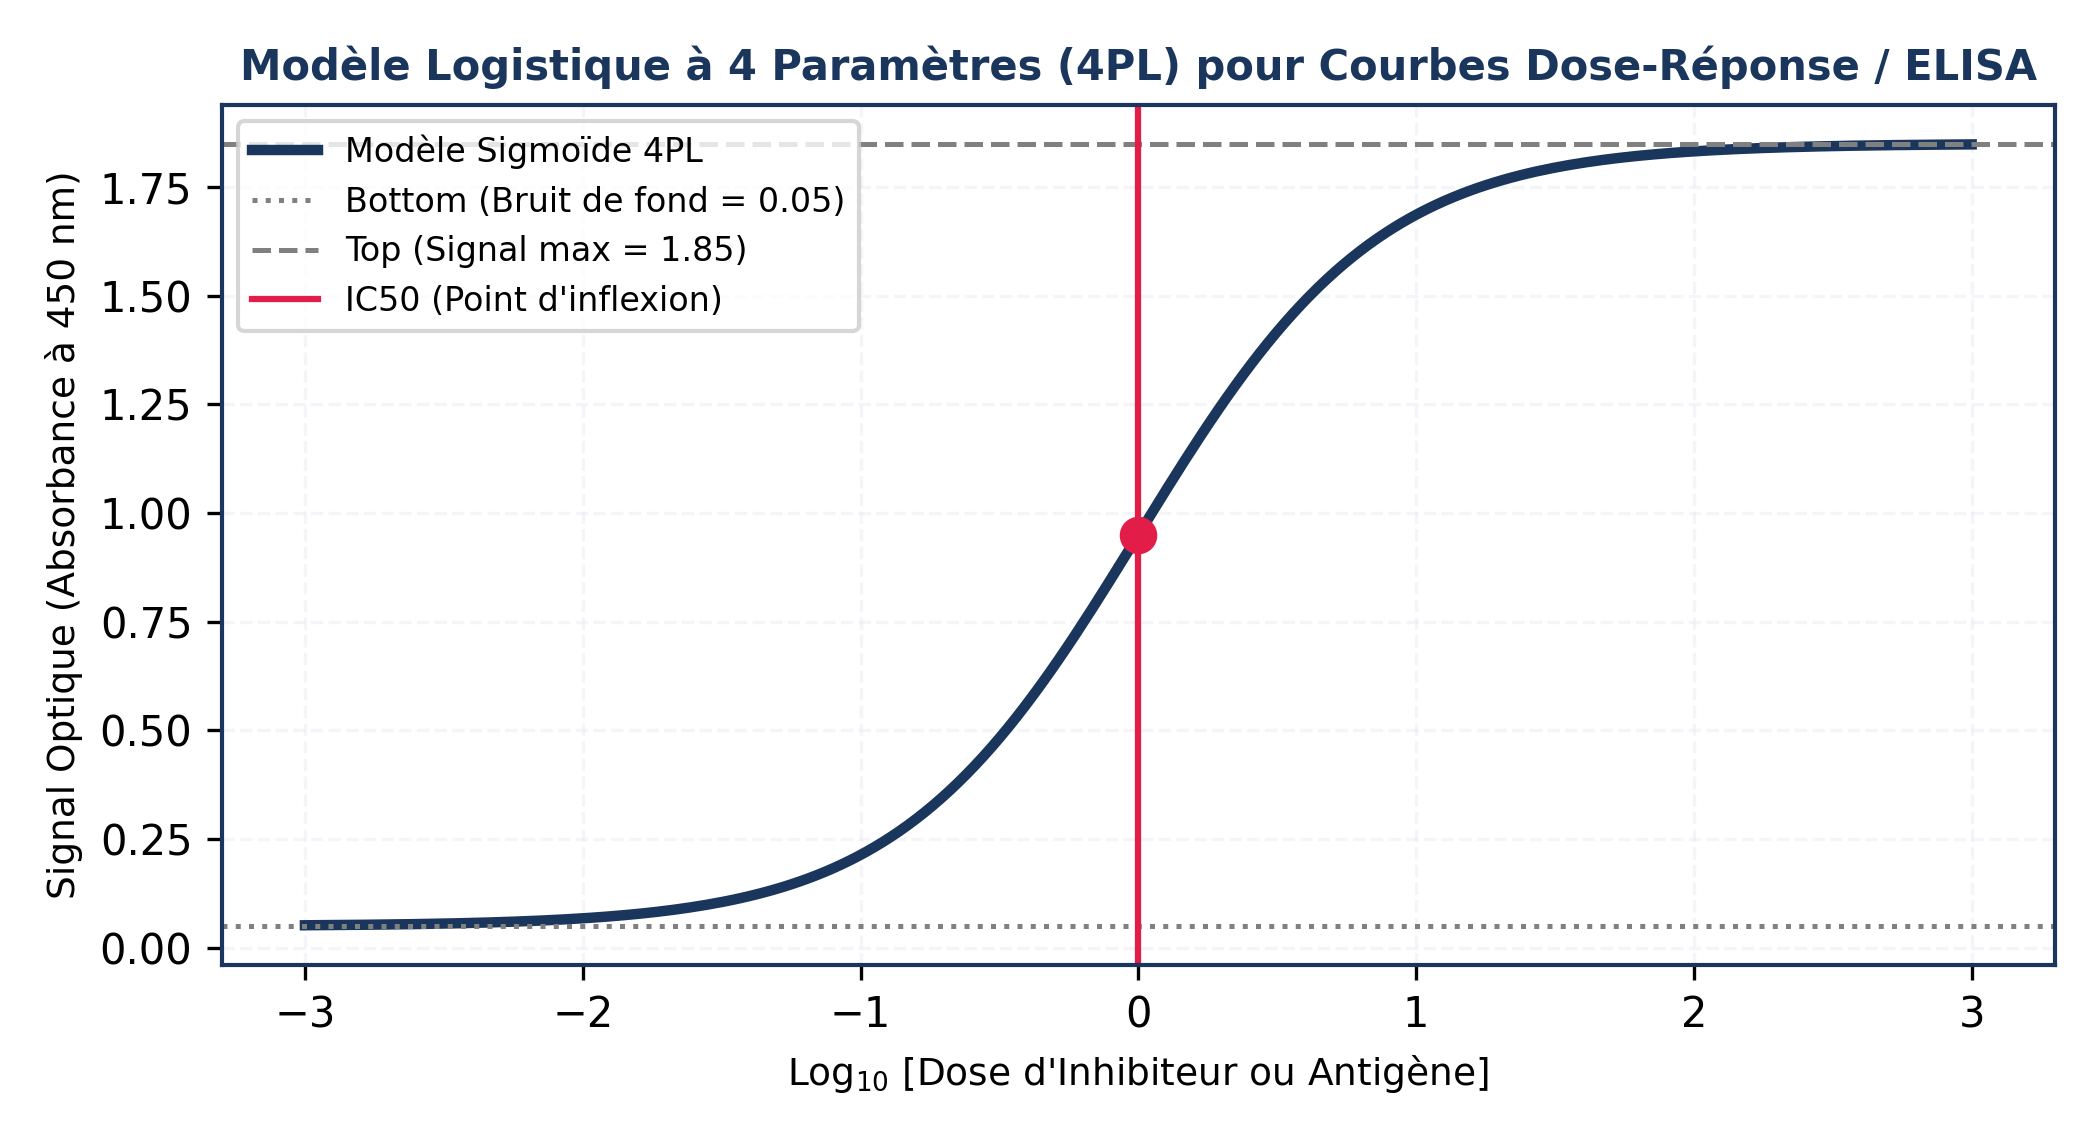
\includegraphics[width=0.86\linewidth]{../../sources/figures/fig04_sigmoidal_4pl_elisa.png}
\end{center}
\textbf{Analyse des profils sigmoïdes non linéaires :}
\begin{itemize}[leftmargin=*, label=\faAngleRight]
  \item \textbf{Modèle 4PL d'ELISA (Gauche) :} La zone centrale quasi-rectiligne entourant le point $C = EC_{50}$ définit la \textbf{plage dynamique de dosage}. En dehors de cette zone (plateaux $A$ et $D$), la méthode perd toute sensibilité : une grande variation de concentration n'entraîne quasiment aucune modification du signal optique.
  \item \textbf{Modèle de Hill (Droite) :} Comparaison des profils pour $n_H = 0.5$, $n_H = 1$ (hyperbole michaelienne), et $n_H = 2$ ou $4$. Plus le coefficient de Hill $n_H$ est élevé, plus la courbe prend un aspect vertical abrupt (« interrupteur moléculaire »).
\end{itemize}
\end{figurebox}

\section{Exercices d'Application \& Solutions}

\begin{exercicebox}{Exercice 1 : Cinétique Enzymatique (Michaelis-Menten vs Lineweaver-Burk)}
Une étude sur la phosphatase alcaline mesure la vitesse initiale $v$ ($\mu\text{mol}\cdot\text{min}^{-1}\cdot\text{mg}^{-1}$) pour 6 concentrations de substrat $p\text{NPP}$ ($[S]$ en mM) :
\begin{center}
\small
\begin{tabular}{lcccccc}
\toprule
\textbf{$[S]$ (mM)} & 0.20 & 0.50 & 1.00 & 2.50 & 5.00 & 10.00 \\
\textbf{$v$ (mesurée)} & 8.5 & 16.2 & 23.8 & 32.1 & 36.8 & 39.5 \\
\bottomrule
\end{tabular}
\end{center}
L'ajustement non linéaire direct (NLLS) sous Python fournit :
\begin{equation*}
  \hat{V}_{\max} = 43.80 \pm 0.75\,\mu\text{mol}\cdot\text{min}^{-1}\cdot\text{mg}^{-1}, \qquad \hat{K}_m = 0.840 \pm 0.045\,\text{mM}
\end{equation*}
La valeur critique de Student pour $df = 6 - 2 = 4$ est $t_{0.05}(4) = 2.776$.
\begin{enumerate}[label=\textbf{\alph*.}]
  \item Calculez les doubles réciproques $1/[S]$ et $1/v$ pour le point 1 ($[S] = 0.20$) et le point 6 ($[S] = 10.00$).
  \item Calculez l'intervalle de confiance à 95\% du paramètre d'affinité $\hat{K}_m$.
  \item Calculez la vitesse initiale théorique prédite à $[S] = 0.840\,\text{mM}$ et à $[S] = 10.0\,\text{mM}$.
  \item Une mutation génétique du site catalytique donne $\hat{K}_m = 4.20\,\text{mM}$. Quelle est la conséquence biologique sur l'affinité enzymatique ?
\end{enumerate}
\end{exercicebox}

\begin{solutionbox}{Solution : Exercice 1}
\begin{enumerate}[label=\textbf{\alph*.}]
  \item \textbf{Calcul des doubles réciproques :}
  \begin{itemize}
    \item Point 1 : $\frac{1}{[S]} = \frac{1}{0.20} = \mathbf{5.00\,\text{mM}^{-1}}$, \quad $\frac{1}{v} = \frac{1}{8.5} = \mathbf{0.1176}$.
    \item Point 6 : $\frac{1}{[S]} = \frac{1}{10.00} = \mathbf{0.10\,\text{mM}^{-1}}$, \quad $\frac{1}{v} = \frac{1}{39.5} = \mathbf{0.0253}$.
  \end{itemize}
  \item \textbf{Intervalle de confiance à 95\% de $K_m$ :}
  \begin{align*}
    IC_{95\%}(K_m) &= 0.840 \pm \left( 2.776 \times 0.045 \right) \\
    &= 0.840 \pm 0.125 = \mathbf{[0.715 \,;\, 0.965]\,\text{mM}}
  \end{align*}
  \item \textbf{Vitesses théoriques prédites :}
  \begin{itemize}
    \item Pour $[S] = K_m = 0.840\,\text{mM}$ :
    \begin{equation*}
      v = \frac{43.80 \times 0.840}{0.840 + 0.840} = \frac{43.80}{2} = \mathbf{21.90\,\mu\text{mol}\cdot\text{min}^{-1}\cdot\text{mg}^{-1}}
    \end{equation*}
    \item Pour $[S] = 10.0\,\text{mM}$ :
    \begin{equation*}
      v = \frac{43.80 \times 10.0}{0.840 + 10.0} = \frac{438.0}{10.840} = \mathbf{40.41\,\mu\text{mol}\cdot\text{min}^{-1}\cdot\text{mg}^{-1}}
    \end{equation*}
  \end{itemize}
  \item \textbf{Conséquence biologique de la mutation :}
  Puisque le $K_m$ passe de $0.840\,\text{mM}$ à $4.20\,\text{mM}$ (multiplié par 5), \textbf{l'affinité apparente de l'enzyme mutée pour son substrat est fortement diminuée}. Il faut une concentration de substrat 5 fois plus élevée pour atteindre la demi-vitesse maximale.
\end{enumerate}
\end{solutionbox}

\begin{exercicebox}{Exercice 2 : Modélisation Allostérique de Hill (PFK-1 Hépatique)}
L'activité de la phosphofructokinase-1 (PFK-1) hépatique mesurée en fonction de la concentration en fructose-6-phosphate ($[S]$ en mM) fournit par NLLS les paramètres de Hill suivants :
\begin{equation*}
  \hat{V}_{\max} = 120.0\,\text{U/mg}, \qquad \hat{K}_{0.5} = 2.00\,\text{mM}, \qquad \hat{n}_H = 2.80
\end{equation*}
\begin{enumerate}[label=\textbf{\alph*.}]
  \item Que signifie biologiquement $\hat{n}_H = 2.80$ ?
  \item Calculez la vitesse initiale pour $[S] = 1.00\,\text{mM}$ (moitié de $K_{0.5}$) et $[S] = 2.00\,\text{mM}$ ($[S] = K_{0.5}$).
  \item Calculez le ratio $v(2\,\text{mM}) / v(1\,\text{mM})$. Comparez ce saut avec ce qu'aurait donné une cinétique purement michaelienne ($n_H = 1$).
  \item Pourquoi parle-t-on d'effet « interrupteur biologique » ?
\end{enumerate}
\end{exercicebox}

\begin{solutionbox}{Solution : Exercice 2}
\begin{enumerate}[label=\textbf{\alph*.}]
  \item \textbf{Signification biologique de $n_H = 2.80$ :}
  Puisque $\hat{n}_H = 2.80 > 1$, la PFK-1 présente une \textbf{coopérativité allostérique positive marquée}. La fixation d'un substrat sur l'une des sous-unités induit un changement conformationnel qui augmente considérablement l'affinité des sous-unités adjacentes.
  \item \textbf{Calculs des vitesses :}
  \begin{itemize}
    \item À $[S] = 2.00\,\text{mM} = K_{0.5}$ :
    Par définition de $K_{0.5}$, $v = \frac{V_{\max}}{2} = \frac{120.0}{2} = \mathbf{60.0\,\text{U/mg}}$.
    \item À $[S] = 1.00\,\text{mM}$ :
    \begin{align*}
      [S]^{2.80} &= 1.00^{2.80} = 1.000 \\
      K_{0.5}^{2.80} &= 2.00^{2.80} \approx 6.964 \\
      v &= \frac{120.0 \times 1.000}{6.964 + 1.000} = \frac{120.0}{7.964} = \mathbf{15.07\,\text{U/mg}}
    \end{align*}
  \end{itemize}
  \item \textbf{Amplification de la réponse :}
  Le ratio de vitesse lorsque $[S]$ double (de 1 à 2 mM) est de :
  \begin{equation*}
    \frac{v(2\,\text{mM})}{v(1\,\text{mM})} = \frac{60.0}{15.07} \approx \mathbf{3.98} \quad (\text{Facteur 4 !})
  \end{equation*}
  Pour une enzyme michaelienne classique ($n_H = 1$), on aurait eu $v(1) = 120 \times \frac{1}{3} = 40$ et $v(2) = 60$, soit un ratio de seulement $\frac{60}{40} = \mathbf{1.50}$.
  \item \textbf{Concept d'interrupteur métabolique :}
  Grâce à la coopérativité allostérique, une faible variation physiologique du substrat active massivement la voie de la glycolyse sans nécessiter une hausse démesurée des concentrations métaboliques.
\end{enumerate}
\end{solutionbox}

\section*{Formulaire Récapitulatif : Modèles Non Linéaires}
\begin{center}
\resizebox{\linewidth}{!}{%
\begin{tabular}{lll}
\toprule
\textbf{Modèle Biologique} & \textbf{Équation Mathématique} & \textbf{Paramètres Clés \& Application} \\
\midrule
Michaelis-Menten & $v = \frac{V_{\max} [S]}{K_m + [S]}$ & $V_{\max}$ (vitesse limite), $K_m$ (affinité inverse) \\
Modèle Allostérique de Hill & $v = \frac{V_{\max} [S]^{n_H}}{K_{0.5}^{n_H} + [S]^{n_H}}$ & $n_H > 1$ (coopérativité positive, sigmoïde) \\
Modèle Logistique 4PL (ELISA) & $y = D + \frac{A - D}{1 + (x/C)^B}$ & $A$ (bruit), $D$ (saturation), $C$ ($EC_{50}$), $B$ (pente) \\
Moindres Carrés Non Linéaires & $\min \sum (y_i - f(x_i; \theta))^2$ & Résolu par Levenberg-Marquardt (sans distorsion) \\
\bottomrule
\end{tabular}%
}
\end{center}

\end{document}
